% Vize sunumu, model kismi (IP3). Derlemek icin: ./derle.sh  ->  sunum.pdf
% Sayilar experiments/ altindaki JSON kayitlarindan, sekiller rapor klasorunden geliyor.
\documentclass[aspectratio=169,11pt]{beamer}

\usepackage[utf8]{inputenc}
\usepackage[T1]{fontenc}
\usepackage{graphicx}
\usepackage{booktabs}

\graphicspath{{../rapor-latex/grafik/}}

\usetheme{default}
\usefonttheme{professionalfonts}
\setbeamertemplate{navigation symbols}{}
\setbeamertemplate{footline}{\hfill\insertframenumber\,/\,\inserttotalframenumber\hspace{4mm}\vspace{3mm}}
\setbeamertemplate{itemize items}[circle]
\definecolor{lacivert}{RGB}{20,50,95}
\setbeamercolor{frametitle}{fg=lacivert}
\setbeamercolor{title}{fg=lacivert}
\setbeamercolor{structure}{fg=lacivert}
\setbeamerfont{frametitle}{series=\bfseries}
\setlength{\leftmargini}{1.2em}

\title{Türk İşaret Dili Tanıma: Model Eğitimi ve Karşılaştırma}
\subtitle{Bitirme Projesi Ara Raporu, İş Paketi 3}
\author{Mustafa Göktepe \\[1mm] {\small Ekip: Ahmet Çelik, Mustafa Küpeli \quad Danışman: Ar.\ Gör.\ Hayri Öztürk}}
\institute{Erciyes Üniversitesi, Bilgisayar Mühendisliği}
\date{Kasım 2026}

\begin{document}

\begin{frame}[plain]
\titlepage
\end{frame}

% 1
\begin{frame}{Videodan kelimeye giden hat}
\centering
\footnotesize
\setlength{\fboxsep}{4pt}
\fbox{Video} $\rightarrow$
\fbox{MediaPipe} $\rightarrow$
\fbox{Normalizasyon} $\rightarrow$
\fbox{$64\times100$ girdi} $\rightarrow$
\fbox{Model} $\rightarrow$
\fbox{226 kelime}

\vspace{6mm}
\normalsize
\begin{columns}[T]
\begin{column}{0.48\textwidth}
\textbf{Veri: AUTSL}
\begin{itemize}
\item 226 işaret, 43 işaretçi, 36.302 video
\item Eğitim 28.132, doğrulama 4.418, test 3.741
\item Bölmeler işaretçi bazında ayrık
\end{itemize}
\end{column}
\begin{column}{0.48\textwidth}
\textbf{Kare başına 100 sayı}
\begin{itemize}
\item İki el $\times$ 21 nokta, gövde 7 nokta ($x$, $y$)
\item Omuz ortasına ötele, omuz genişliğine böl
\item Her video 64 kareye örneklenir
\end{itemize}
\end{column}
\end{columns}
\end{frame}

% 2
\begin{frame}{Karşılaştırılan iki mimari}
\centering
\begin{tabular}{@{}lll@{}}
\toprule
 & \textbf{BiGRU-2x256} & \textbf{1B-CNN + Transformer} \\
\midrule
Yapı & 2 katman, iki yönlü GRU & 3 evrişim + 2 Transformer katmanı \\
Zaman bilgisi & Kare kare, ileri ve geri & Yerel evrişim, sonra dikkat \\
Dizi uzunluğu & 64 & 64 $\rightarrow$ 32 (stride 2) \\
Çıkış & Zaman ortalaması + doğrusal & Zaman ortalaması + doğrusal \\
Parametre & 2.114.018 & 1.473.634 \\
\bottomrule
\end{tabular}

\vspace{6mm}
\begin{itemize}
\item BiGRU temel model; mobil uygulamada çalışan sürüm bu.
\item İkinci model yüzde 30 daha küçük ve tekrarlayan katmanı yok.
\end{itemize}
\end{frame}

% 3
\begin{frame}{Eğitim düzeni}
\begin{columns}[c]
\begin{column}{0.36\textwidth}
\small
\begin{itemize}
\item İki modelde aynı ayarlar
\item 60 epoch, AdamW, lr $2\times10^{-3}$
\item Kosinüs azaltım, batch 128
\item Etiket yumuşatma 0,1
\item Artırma: kare seyreltme, kırpma, döndürme, ölçek
\item Test kümesi eğitim bitince bir kez ölçüldü
\end{itemize}
\end{column}
\begin{column}{0.62\textwidth}
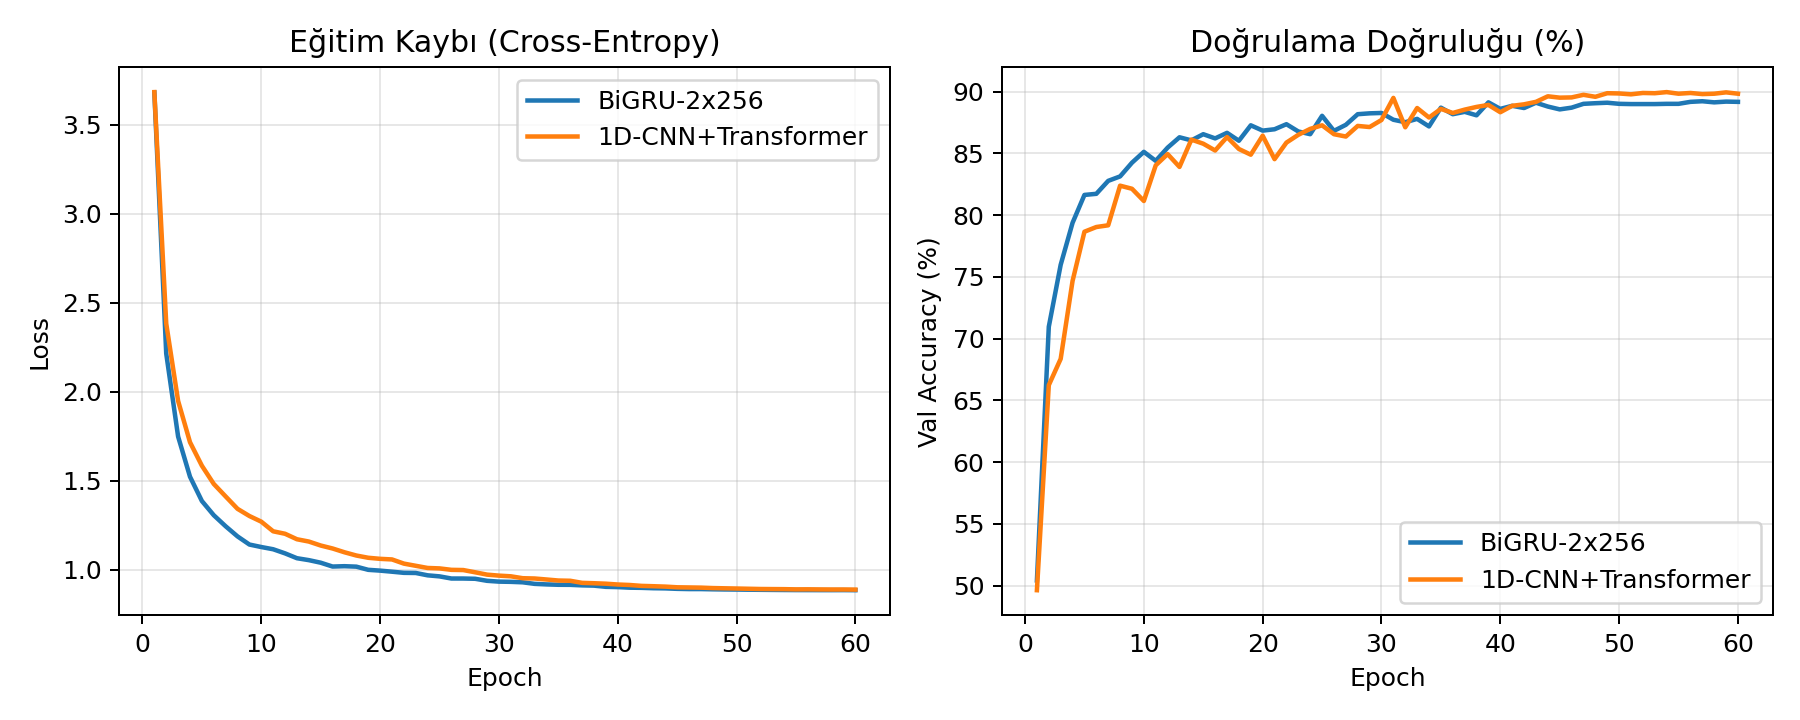
\includegraphics[width=\textwidth]{egitim_egrisi.png}
\end{column}
\end{columns}
\end{frame}

% 4
\begin{frame}{Sonuçlar (226 sınıf, test kümesi)}
\centering
\begin{tabular}{@{}lrrrr@{}}
\toprule
\textbf{Model} & \textbf{Parametre} & \textbf{Doğrulama (\%)} & \textbf{Test (\%)} & \textbf{Macro F1 (\%)} \\
\midrule
BiGRU-2x256 & 2.114.018 & 89,23 & 88,24 & 88,09 \\
1B-CNN + Transformer & 1.473.634 & \textbf{89,97} & \textbf{88,83} & \textbf{88,61} \\
\bottomrule
\end{tabular}

\vspace{2mm}
{\footnotesize Tek koşu, tohum 0 (ara rapor Tablo 2)}

\vspace{5mm}
\begin{tabular}{@{}lrr@{}}
\toprule
\textbf{Üç tohum (0, 1, 2)} & \textbf{Test ort.\ $\pm$ ss (\%)} & \textbf{Doğrulama ort.\ (\%)} \\
\midrule
BiGRU-2x256 & 87,98 $\pm$ 0,23 & 89,38 \\
1B-CNN + Transformer & \textbf{89,42 $\pm$ 0,52} & \textbf{90,37} \\
\bottomrule
\end{tabular}

\vspace{4mm}
\begin{itemize}
\item Yüzde 85 hedefi iki modelde de aşıldı.
\item Küçük model üç tohumun üçünde de önde; eğitimi yaklaşık dört kat hızlı.
\end{itemize}
\end{frame}

% 5
\begin{frame}{Hatalar nerede toplanıyor?}
\begin{columns}[c]
\begin{column}{0.42\textwidth}
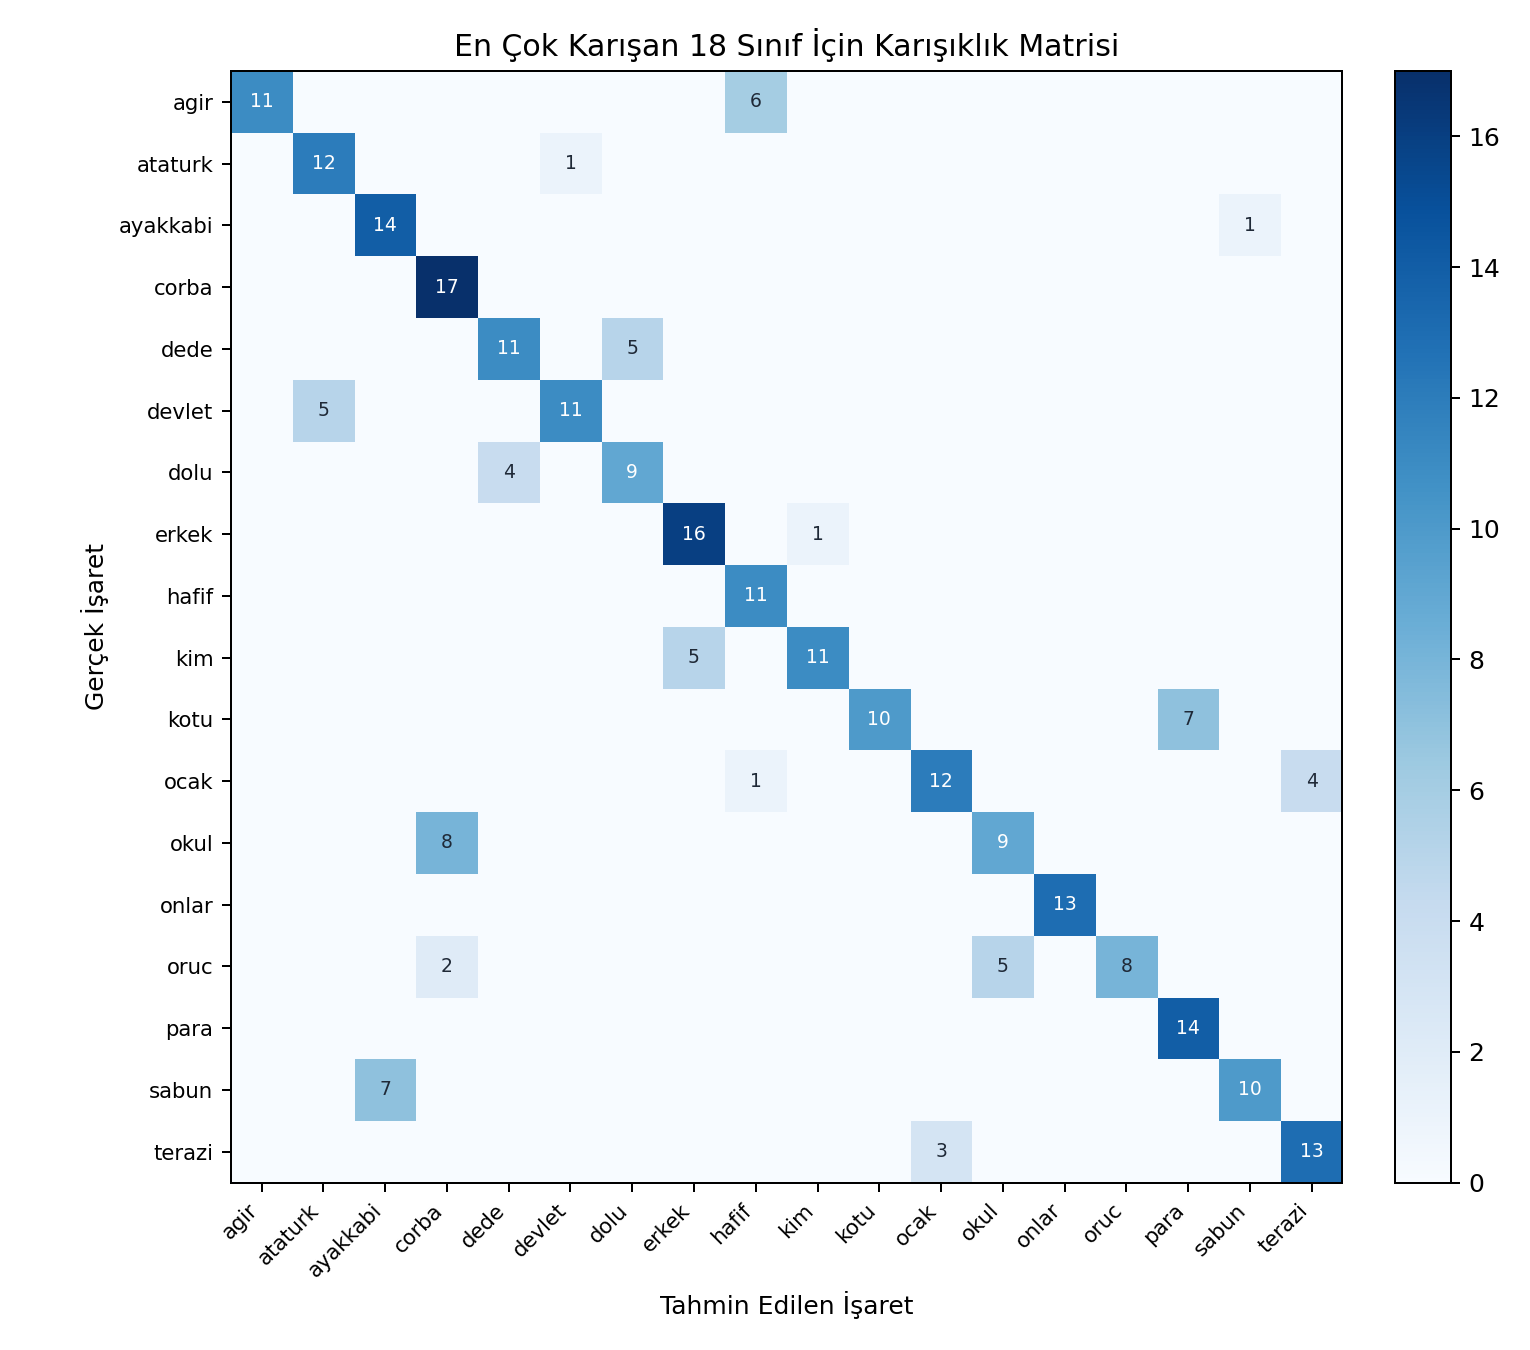
\includegraphics[width=\textwidth]{karisiklik_matrisi.png}
\end{column}
\begin{column}{0.56\textwidth}
\small
\begin{tabular}{@{}llr@{}}
\toprule
\textbf{Gerçek} & \textbf{Tahmin} & \textbf{Hata} \\
\midrule
okul & çorba & 8 / 17 \\
kötü & para & 7 / 17 \\
sabun & ayakkabı & 7 / 17 \\
ağır & hafif & 6 / 17 \\
\bottomrule
\end{tabular}

\vspace{4mm}
\begin{itemize}
\item Hatalar rastgele değil: el formu ve konumu aynı olan işaretler karışıyor.
\item Ayırt eden şey parmak teması ya da derinlik; 2B noktalarda görünmüyor.
\end{itemize}
\end{column}
\end{columns}
\end{frame}

% 6
\begin{frame}{Mobil tarafa aktarım ve sıradaki işler}
\begin{columns}[T]
\begin{column}{0.48\textwidth}
\textbf{Tamamlanan}
\begin{itemize}
\item BiGRU int8 LiteRT: 9,43 MB $\rightarrow$ 3,19 MB, test yüzde 88,0
\item Python ile telefon tahminleri yüzde 99,5 aynı
\item Model çıkarımı 48 ms
\item Güven eşiği 0,6: örneklerin yüzde 75'i kabul, bunlarda doğruluk yüzde 96,8
\end{itemize}
\end{column}
\begin{column}{0.48\textwidth}
\textbf{Açık konular}
\begin{itemize}
\item Canlı kamerada güven düşük; veri setindeki videolarla fark inceleniyor
\item Uçtan uca hız yaklaşık 9 FPS, darboğaz MediaPipe
\item 1B-CNN + Transformer'ın mobil dönüşümü
\item Sürekli işaretlemede segmentleme
\end{itemize}
\end{column}
\end{columns}
\end{frame}

\end{document}
